\subsection{Quartic Harmonic Oscillator}
\label{sec:qosc_results}

The quartic harmonic oscillator \cite{PhysRev.184.1231, girguś2024spiralflowquantumquartic, wójcik2012applicationnumericalrenormalizationgroup} is an extension of the standard harmonic oscillator with an additional non-linearity of the form $g \varphi^4$, where $g$ is an arbitrary constant that dictates the strength of the interaction, and $\phi$ is a bosonic field.
This leads to the Hamiltonian $H = \frac12\dot\phi^2 + \frac{m}{2}\phi^2 + gm^3\phi^4 $, where $\phi$ is composed of a single mode.
$m$ is the mass of the bosonic particle, and $\dot \phi$ represents the time derivate of the field.

In a second-quantized, dimensionless form, the Hamiltonian can be written as:
\begin{equation}
    \label{eq:qosc}
    H = a^\dagger a + g\left(a + a^\dagger \right)^4
\end{equation}
where there is only one bosonic mode.

After expanding the product, normal ordering all terms, and removing the constant offset, this Hamiltonian can be written as a linear combination of $8$ terms consisting of three pairs of operators plus their Hermitian conjugates and two operators that are their own Hermitian conjugates:
\begin{equation}
    \begin{split}
        H = &(12g + 1) a^\dagger a + 6g a^{\dagger^2} a^2 + 6g \left(a^{\dagger^2} + a^2 \right) \\
        + &4g \left(a^{\dagger^3} a + a^\dagger a^3 \right) + g \left(a^{\dagger^4} + a^4 \right)
    \end{split}
\end{equation}

\begin{figure*}
    \label{fig:qosc}
    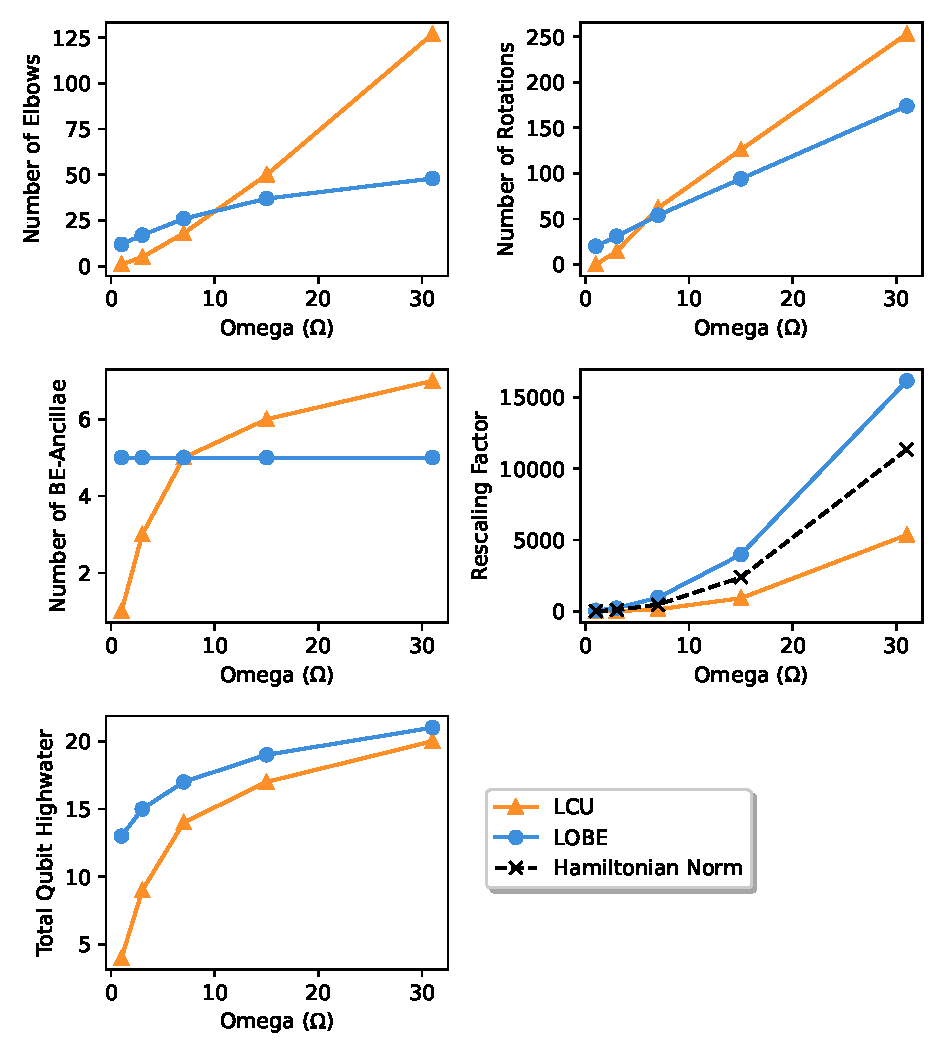
\includegraphics[width = 16cm]{figures/quartic_oscillator.pdf}
    \caption{
        \textbf{Quartic Harmonic Oscillator}
        The number of T gates (upper-left), number of non-Clifford rotations (lower-left), block-encoding ancillae (upper-middle), maximum number of qubits used (lower-middle), and rescaling factor (lower-right) are shown as a function of the bosonic occupation cutoff ($\Omega$).
        The parameter $g$ is set to $1$ for all data points.
        Results for the Pauli Expansion method are shown as the orange triangles and results for LOBE are shown as the blue circles.
        The L2 norm of the Hamiltonian is shown as the dashed black crosses.
    }
\end{figure*}

In Figure \ref{fig:qosc}, we show the scaling of the spacetime costs associated with both the LOBE and Pauli Expansion block-encodings as a function of the bosonic occupation cutoff ($\Omega$).
For small values of $\Omega$, the Pauli Expansion block-encodings result in lower spacetime costs, however, the LOBE constructions have favorable scaling and therefore a crossover point is seen.

For the time-complexity, this crossover occurs at $\Omega = 15$ for the number of T gates and $\Omega = 7$ for the number of non-Clifford rotations.
For the space-complexity, this crossover occurs at $\Omega = 7$ for the number of block-encoding ancillae and $\Omega = 31$ for the maximum number of qubits.
Finally, for the rescaling factor, this crossover occurs at $\Omega = 31$.
